% THIS IS SIGPROC-SP.TEX - VERSION 3.1
% WORKS WITH V3.2SP OF ACM_PROC_ARTICLE-SP.CLS
% APRIL 2009
%
% It is an example file showing how to use the 'acm_proc_article-sp.cls' V3.2SP
% LaTeX2e document class file for Conference Proceedings submissions.
% ----------------------------------------------------------------------------------------------------------------
% This .tex file (and associated .cls V3.2SP) *DOES NOT* produce:
%       1) The Permission Statement
%       2) The Conference (location) Info information
%       3) The Copyright Line with ACM data
%       4) Page numbering
% ---------------------------------------------------------------------------------------------------------------
% It is an example which *does* use the .bib file (from which the .bbl file
% is produced).
% REMEMBER HOWEVER: After having produced the .bbl file,
% and prior to final submission,
% you need to 'insert'  your .bbl file into your source .tex file so as to provide
% ONE 'self-contained' source file.
%
% Questions regarding SIGS should be sent to
% Adrienne Griscti ---> griscti@acm.org
%
% Questions/suggestions regarding the guidelines, .tex and .cls files, etc. to
% Gerald Murray ---> murray@hq.acm.org
%
% For tracking purposes - this is V3.1SP - APRIL 2009

\documentclass{acm_proc_article-sp}

\begin{document}

\title{An Investigation of the Effects of Mental Fatigue on Programming Tasks'
Performance}

\numberofauthors{2} %  in this sample file, there are a *total*

\author{
% You can go ahead and credit any number of authors here,
% e.g. one 'row of three' or two rows (consisting of one row of three
% and a second row of one, two or three).
%
% The command \alignauthor (no curly braces needed) should
% precede each author name, affiliation/snail-mail address and
% e-mail address. Additionally, tag each line of
% affiliation/address with \affaddr, and tag the
% e-mail address with \email.
%
% 1st. author
\alignauthor
Saurabh Sarkar\\
       \affaddr{Department of Computer Science}\\
       \affaddr{North Carolina State University}\\
       \affaddr{Raleigh, NC}\\
       \email{ssarkar4@ncsu.edu}
% 2nd. author
\alignauthor
Chris Parnin\\
       \affaddr{Department of Computer Science}\\
       \affaddr{North Carolina State University}\\
       \affaddr{Raleigh, NC}\\
       \email{cjparnin@ncsu.edu}
}

\maketitle
\begin{abstract}
Mental fatigue reduces the cognitive and physical performance of people. 
I propose to investigate how mental fatigue affects programmers to perform 
poor in software industries, causing system developed by them to fail in the 
long run. This project is the part of my thesis research project with 
\textit{Dr. Parnin}\footnote{http://www.chrisparnin.me/}. We will be
validating our hypothesis with the help of surveys and user studies. 
This project is to define the research guidelines to further investigate
different methods to automatically determine the fatigue level of programmers.  
We can use this information to help programmers avoid their fatigue state to
control errors in programming, and eventually aid them to be more productive.
\end{abstract}

\keywords{Software Engineering, Psychology, Fatigue, Work Environment} % NOT
% required for Proceedings

\section{Introduction}
Fatigue is a physiological state of reduced mental or physical mental
capability. Fatigue is always ambiguous to be defined. It results from excessive
workload(both physical and mental), exhaustion, or sleeploss. Fatigue (also
called exhaustion, tiredness, lethargy, languidness, languor, lassitude, and
listlessness) \cite{website:wiki-fatigue} is a complex happening and have all
physiological and psychological characterisctics \cite{psychology:paul}. Fatigue
can be categorized accordin to its effects and distinctiveness. Workload causes
muscle pain and bruning sensation in body. The inability to perform any physical
activities at the level of one's normal activities is \textit{physical/muscular
fatigue}. \textit{Mental fatigue} is defined as a state of weariness, with a
feeling of boredom/saturation and declines motivation \cite{lauren:defining}.
Fatigue is one of the 13 mood states \cite{stone:fatigue}. Stress causes
emotions and mood swings. Dull emotional responses is cahracterized as
\textit{Emotional Fatigue}. People have capabilities of doing certain tasks.
\textit{Skills Fatigue} deals with their ability to perform those tasks. People
are susceptible to fatigue and its effects, that hamper their daily activities,
their ability to perform and ultimately affects the results.

Mental fatigue is caused due to exhaustion and tiredness, triggered by long and
demanding tasks \cite{lauren:defining}. Exhaustion due to extreme mental and
physical work causes performance degradation in execution of human tasks.
Mental fatigue also has a negative effect on memory and cognitive
functionalities and these functionalities play a vital role in program
construction and modeling \cite{schneiderman:interaction}. Mental fatigue is
universal to all software developers \cite{website:blog-fatigue}. Studies have
shown possible relations between mental fatigue and specific programming tasks
such as a program construction, modeling and debugging \cite{schneiderman:interaction}.

Primary reasons for system failures are due to low performance of programmers,
caused by their absentmindedness or exhaustion. Mental fatigue can also lead to
system failures in the long run. Mental fatigue can also lead to system failures
in the long run \cite{rocco:gartner}. Exhaustion due to extreme mental and
physical work causes performance degradation in execution of human tasks. In
today's competitive world, software programmers are motivated to work hard, and
hence keep themselves involved in numerous projects. Sometimes they work in
teams and sometime they work individually on a project. Again, this all lead to
sleepless nights resulting in more exhaustion and tiredness. Several times
programmers suffer from psychological diseases which they themselves are not
aware of \cite{website:blog-fatigue}. Programmers may make mistakes and
therefore introduce bugs during software development. These mental errors are
due to cognitive failures like distraction, low decision making power, less
reasoning capabilities, and poor attention and focus \cite{larson:cogFailures}. 

Tests \cite{saito:industry} quantifies few subjective symptoms of fatigue in
performing general tasks, that relates to programming domain:
  \begin{enumerate}
   		\item Exhausted \& Drowsy
   		\begin{enumerate}
   		  \item Sleepiness
   		  \item Restlessness
   		  \item Feeling tired
   		  \item Sluggish
   		  \item Lethargy
   		\end{enumerate}
   		\item Mental decline
   		\begin{enumerate}
   		  \item Nervousness
   		  \item Unwillingness
   		  \item Lack of focus
   		  \item Absentmindedness
   		  \item Anxiety
   		  \item Weariness
   		\end{enumerate}
   		\item Incongruity in body \& nervous systems
   		\begin{enumerate}
   		  \item Physical Strength
   		  \item Pain in limbs
   		  \item Strain in eyes
   		  \item Dizziness
   		\end{enumerate}
\end{enumerate}

There is not a lot of work done in this problem area, so my approach would be to
create incremental models that can be refined over time with continuous
evaluation of the research. My contribution intends to define some measurements
for measuring the mental fatigue and analyzing its effect on developers'
performance. This is a step towards working to solve the problem of programmers'
mental fatigue affecting various programming tasks in the software development
process. In Section 2, we illustrate the related works in the field of fatigue
and what other cognitive aspects have been researched in programming domain.
Section 3 presents design and limitations of our approach towards the problem.
In Section 4, we discuss the results of our study and give a detailed
analysis of the observations providing a vision of our research. In summary, we
make the following contributions [TODO]:


\section{Related Work}
Empirical studies have been conducted in the cognitive aspects 
of software engineering. Khan et. al. \cite{khan:mood} have worked on the effect 
of programmers' moods on the performance of programming debugging, 
which also comes under the umbrella of psychological causes. 
My approach takes mental fatigue as the psychological factor 
rather than mood and focuses on all the programming tasks than just 
on program debugging. Pimenta et. al.
\cite{pimenta:monitor} \cite{pimenta:analysis} have worked on monitoring and
analyzing the human performance with respect to the computers and the effects 
of fatigue on it. My proposal is the extension of 
this approach by using different ways to analyze the effects of 
fatigue and providing an aid to the programmer. Saito \cite{saito:industry} has worked 
on assessment of physical fatigue in industries. Several works 
have been done on the risk of cognitive incapability of other 
types of work like driving or physical activities in industries, 
however, few works have been done about finding risk in the programming 
tasks of IT personals.

Numerous articles and blogs discuss about the effect of fatigue 
on the efficacy of programmers in tasks like program understanding, 
construction, modeling, debugging and decision making. 
Industries need a tool which can help programmers detect the mental 
fatigue state and work on it.

This proposed project is first of the many steps taken in this 
direction, opening a wider scope for more research in the domain.


\section{Methodologies}
The approach is to validate our hypothesis and then set some research
guidelines to investigate methods to determine fatigue state of programmers. In
order to set the research guideline, few research questions must be answered
first:
\begin{itemize}
  \item RQ1: \textit{How severe and frequent fatigue is a problem for
  programmers?}
  \item RQ2: \textit{What are the factors that lead to mental fatigue state in
  a programmer's life?}
   \item RQ3: \textit{What are the effects of mental fatigue in a programmer's
   life?}
\end{itemize}
We conducted a formative study to get answer these questions.
Additionally, the methodology comprises a case study to try setting some
benchmark, which includes initial experimental validation using an
instrumentation tool (Eclipse plug-in).

\subsection{Validating Hypothesis: Survey}
In order to validate the hypothesis of mental fatigue deteriorting
programmers' performance and to resolve the dilemma of quantifying and measuring
fatigue with respect to the programming tasks, we intend to build a novel model
to classify fatigue and relate it. However, to achieve that, we must set some
guidelines on the basis of which we will be able to quantify and define fatigue.
This will help us answer the above mentioned research questions.

We conducted a survey and got 311 participants to respond. This survey was
distributed with \textit{checkbox.io}\footnote{http://checkbox.io/}.
Participants entered in a drawing for three \$50 gift cards. Links to this
survey were posted on reddit groups, Quora, posted in Computer Science Facebook
groups, and emailed out to list servs that were directed towards software developers.
The age distribution of the participants lies mostly between 20 and 60 [Figure
1]. Repondents' answers helped us gather data about fatigue and investigate
possible detection and alleviation mechanisms. The survey consists of three
parts: questions about sleep habits and fatigue levels, questions about fatigue
and work performance and question about work habits. The survey
questions can be found in Table 1.
  \begin{figure}
	\centering
	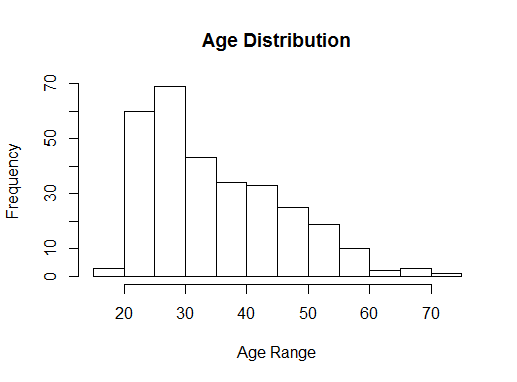
\includegraphics[width=0.5\textwidth,natwidth=517,natheight=382]{age.png}
	\caption{Age distribution of the survey participants.}
  \end{figure}
  \begin{table*}
	\centering
	\caption{Survey Questions}
	\begin{tabular}{|c|c|l|} \hline
		S.No.&Part&Questions\\ \hline
		S1 & Sleep & How many hours do you sleep typically, in a day?\\ \hline
		S2 & & How long did you sleep last night?\\ \hline
		S3 & & What are the factors, you think, lead to mental fatigue in your life
		mostly? \\ \hline S4 & Fatigue at Work & Do you think fatigue is a severe and
		frequent problem for programmers? \\ \hline S5 & & Do you feel when you are
		tired that it influences your performance? If yes, what are some examples? \\
		\hline S6 & & What makes to conclude that your performance is deteriorating or
		you need a break at the moment?\\ \hline S7 & Work & Describe your daily work
		routine. Does this routine occur during the morning, afternoon, or night? \\
		\hline S8 & & What factors might reduce your energy/concentration level as you
		code, throughout the day? \\ \hline S9 & & Age: \\ \hline
		\end{tabular}
	\end{table*}
  
\subsubsection{Results}
The results of our survey show programmers' view towards fatigue. It helped
us identify the factors leading to mental fatigue and it's influence on the
performance of any programming task. In addition, several implications allow us
to speculate on the way programmers behave when they are in the fatigue state.
  \begin{itemize}
  \item Analysis of the survey questions S1-S9 to answer the research
  questions R1-R3 [Sample: Figure 2-4]
   \begin{figure}
	\centering
	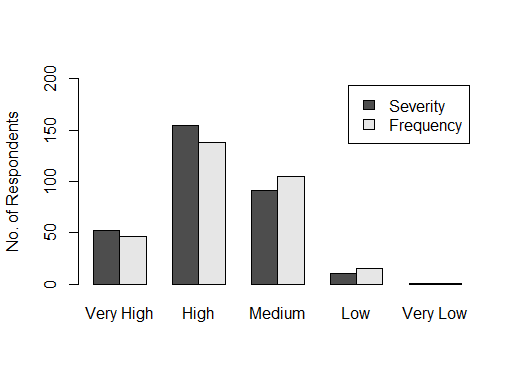
\includegraphics[width=0.5\textwidth,natwidth=517,natheight=382]{sevFreq.png}
	\caption{Severity \& Frequency of fatigue.}
   \end{figure}
   \begin{figure}
	\centering
	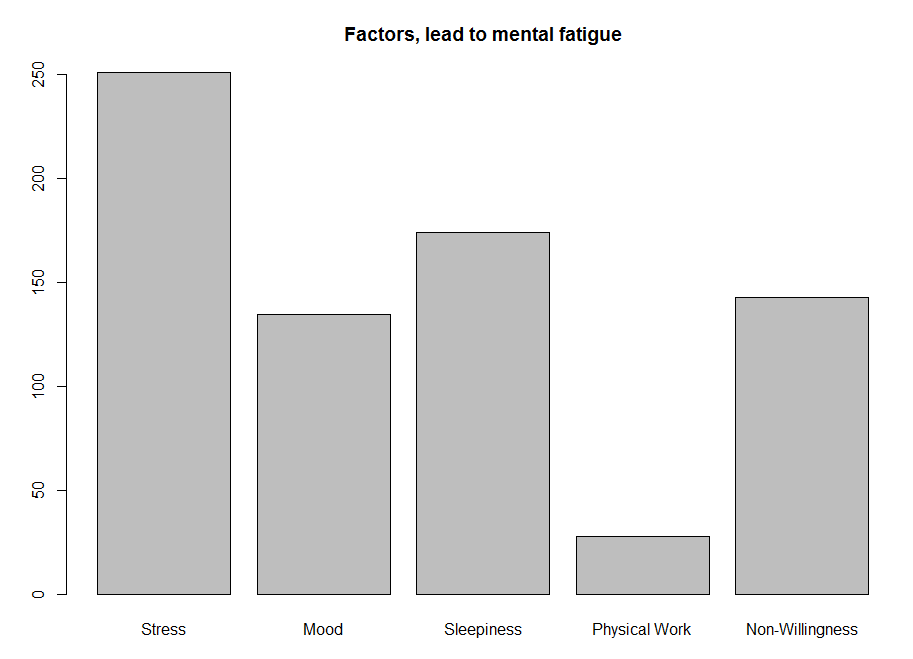
\includegraphics[width=0.5\textwidth,natwidth=913,natheight=659]{factors.png}
	\caption{Factors leading to mental fatigue.}
   \end{figure}
   \begin{figure}
	\centering
	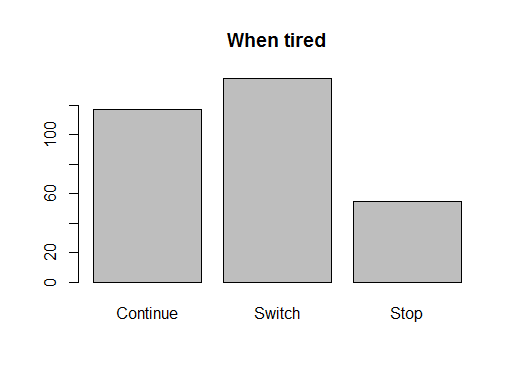
\includegraphics[width=0.5\textwidth,natwidth=517,natheight=382]{tired.png}
	\caption{Actions taken when tired.}
   \end{figure}
  	\begin{enumerate}
   		\item S1
   		\item S2 
   		\item \ldots
    \end{enumerate}
   \begin{figure}
	\centering
	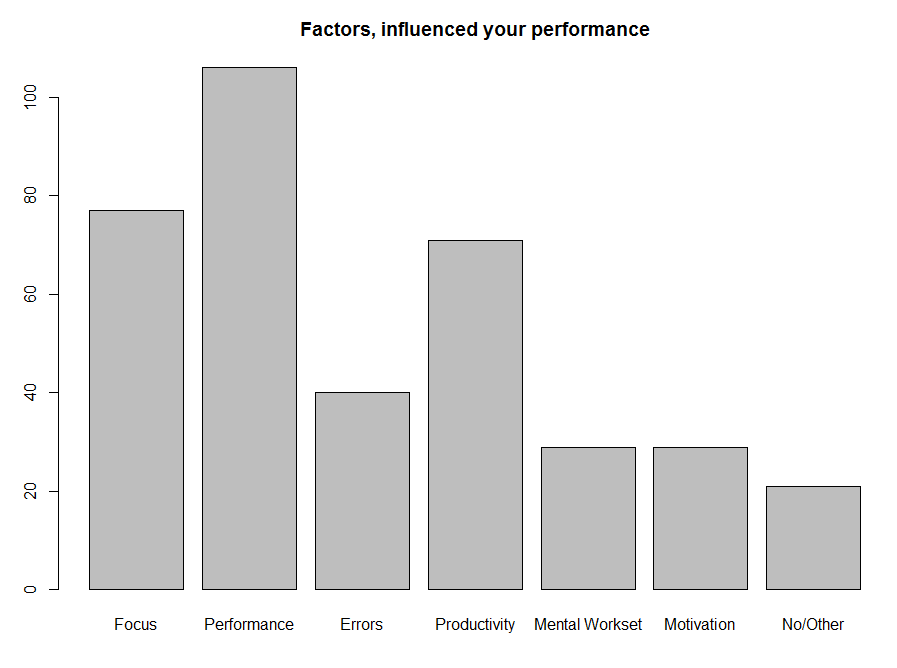
\includegraphics[width=0.5\textwidth,natwidth=913,natheight=659]{influenced.png}
	\caption{Factors influencing the performance.}
   \end{figure}
  \item Implications of the research questions to set guidelines for
  investigation [Sample: Figure 5]
  \item Although our formative study provides data on how programmers think of
  fatigue and how fatgiue affect their performance in programming tasks. There
  are several threats to validity that should be considered when interpreting our results.
  \end{itemize}

\subsection{Experimental Validation: Instrumentation}
To investigate the usefulness of identifying fatigue during programming tasks
and recognizing its impact on the performance, we evaluated the outcome of the
survey study by conducting some other empirical studies of programmers.

We implemented our technique as a plug-in for the Eclipse IDE. DevFatigue is an
activity tracking plug-in for Eclipse. It is an extension of Rabbit \\
\textit{https://code.google.com/p/rabbit-eclipse/}. Alike Rabbit, it works in
the background with Eclipse and tracks all the activities you perform. It only
tracks the actions when Eclipse is active. And logs the data in XML (human
readable) format at specific location. Update site and information URL for
installation: \\
\textit{http://www4.ncsu.edu/~ssarkar4/fatigue/eclipse/updatesite/}

The Rabbit features [content taken from Rabbit Information Page], which it
supports by default:
\begin{itemize}
	\item Commands - How often you use each commands (cut, copy, paste etc), do you
	know which is your favorite?
	\item Editors and Views - Time spent using different
	tool within Eclipse, such as Java Editor, Outline view.
	\item Perspectives - Time spent using different perspectives.
	\item Sessions - Time spent using Eclipse.
	\item Resources - Time spent working on difference resources such as files,
	projects.
	\item Java Elements - Time spent working on Java elements such as classes,
	methods.
	\item Launches - Launches such application runs, debug runs etc, and the
	relevant files will be recorded too when you step into them using the
	debugging.
	\item Task - Time spent working on tasks (tasks in Task List view) and
	resources.
\end{itemize}

Additional features in DevFatigue:
\begin{itemize}
	\item User Activity - The typing speed (key board usage) of the user with
	respect to a time period.
	\item Focus Events - The activities related to keys and mouse usage, like Key
	Up, Key Down, Mouse Clicks, Mouse Velocity, etc. with specific to time period.
	\item Project Events - Information regarding the projects like �imports�, and
	commands used with respect to time period.
\end{itemize}


The architecture of the proposed framework is the extension of the used in some
of the previous studies \cite{pimenta:analysis}.
Indicators of mental fatigue recorded by DevFatigue
  	\begin{enumerate}
   		\item Keydown Time
   		\item Errors per Key Pressed
   		\item Mouse Velocity
   		\item Mouse Acceleration
   		\item Time between Keys
   		\item Double Click Speed
   		\item Number of Double Clicks
   		\item Distance While Clicking etc \ldots
    \end{enumerate}
All the above mentioned indicators have been proved useful in previous studies
\cite{pimenta:monitor} \cite{pimenta:analysis}. These indicators provide us
informations we need to analyze the working patterns of the users and to figure
out any fatigue state in it.

\subsubsection{Hack-a-thons}
Overnight programming competition are always motivating and provides a platform
for programmers to work towards solving a problem. A hackathon is an coding
event where computer programmers collaborate in building a software product.
LexisNexis organized a fall hack-a-thon on 23rd Oct 2014. We approached few of
the participants. All of the participants were graduate students of the Computer
Science department at North Carolina State University (here after refered as
NCSU).

Participants were mostly graduate students in the computer science
department at NCSU. Of the 13 participants invited to participate in the study,
only 2 participants finished the study and turned in the data by DevFatigue.
We collected data using the log files dumped by DevFatigue, and a post-study
questionnaire [Table 2]
	\begin{table*}
		\centering
		\caption{Post-Hackathon Questionnaire}
		\begin{tabular}{|c|c|l|} \hline
			S.No.&Questions\\ \hline
			Q1 & Age?\\ \hline
			Q2 & Any industrial experience?\\ \hline
			Q3 & How would you rate the quality of your code in a scale of 1 to 10, 1
			being the least? \\ \hline
			Q4 & What factors do you think might have affected your performance? \\
			\hline Q5 & Hours slept/rested during the hack-a-thon? \\
			\hline Q6 & Do you think you could have done better, if you had proper rest
			in between? \\ \hline Q7 & Did you win? \\
			\hline
		\end{tabular}
	\end{table*}
\begin{itemize}
  \item Data selection [TODO]
  \item Building a model and classifying mental fatigue [TODO]
  \item Observations from analysis [TODO] \\
      \begin{figure*}
		\centering
		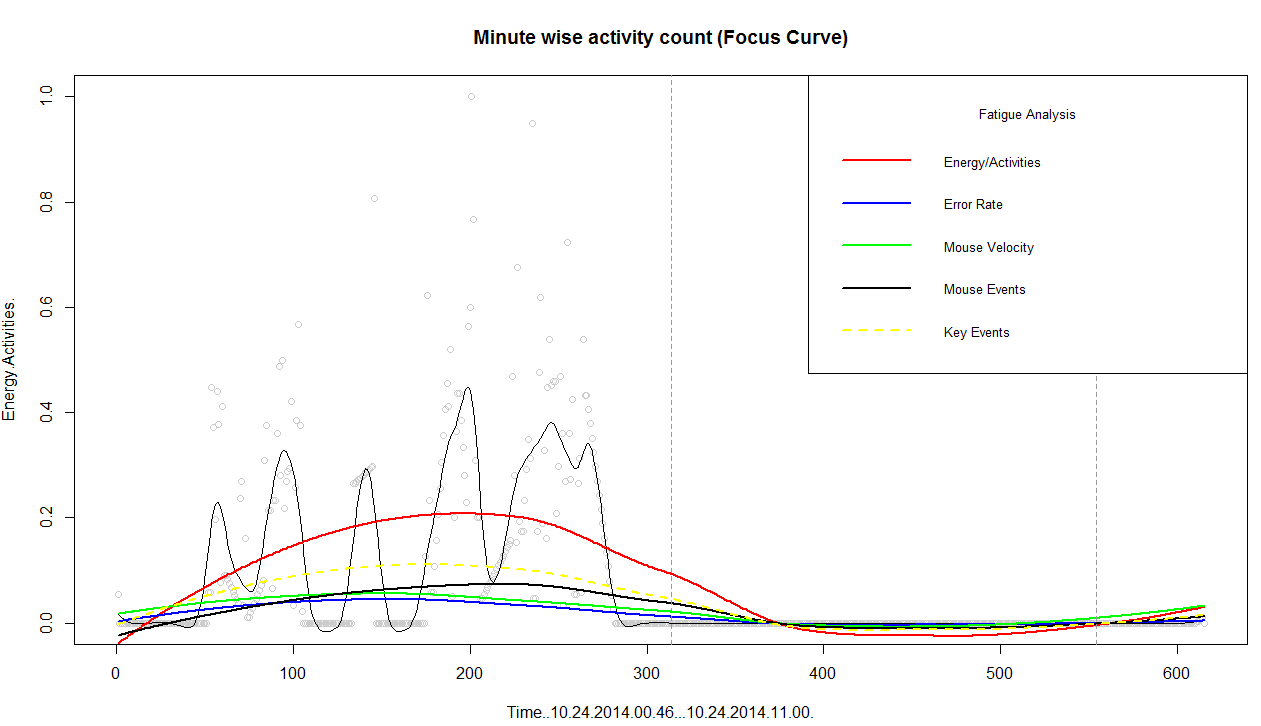
\includegraphics[width=1\textwidth,natwidth=1261,natheight=726]{focusCurveHack.png}
		\caption{Focus Curve - Hack-a-thon Data.}
  	  \end{figure*}
  We intend to come up with a focus curve [Figure 6] that can show some
  working pattern of the user and build a model based on the data collected to
  classify fatigue depending on the user's activities.
\end{itemize}

\subsubsection{In class study}
Dr. Parnin is teaching CSC 510 Software Engineering in Fall 2014 at NCSU. Most
students in the course have some coding experience. Dr. Parnin asked the
students to install DevFatigue and let it track their activies on Eclipse, for a
time-period. In addition, we asked them to log their daily sleep hours. Of the
100 students enrolled in the course, 4 [till now] students responded against
the extra credit offered in the course.
\begin{itemize}
  	  \begin{figure*}
		\centering
		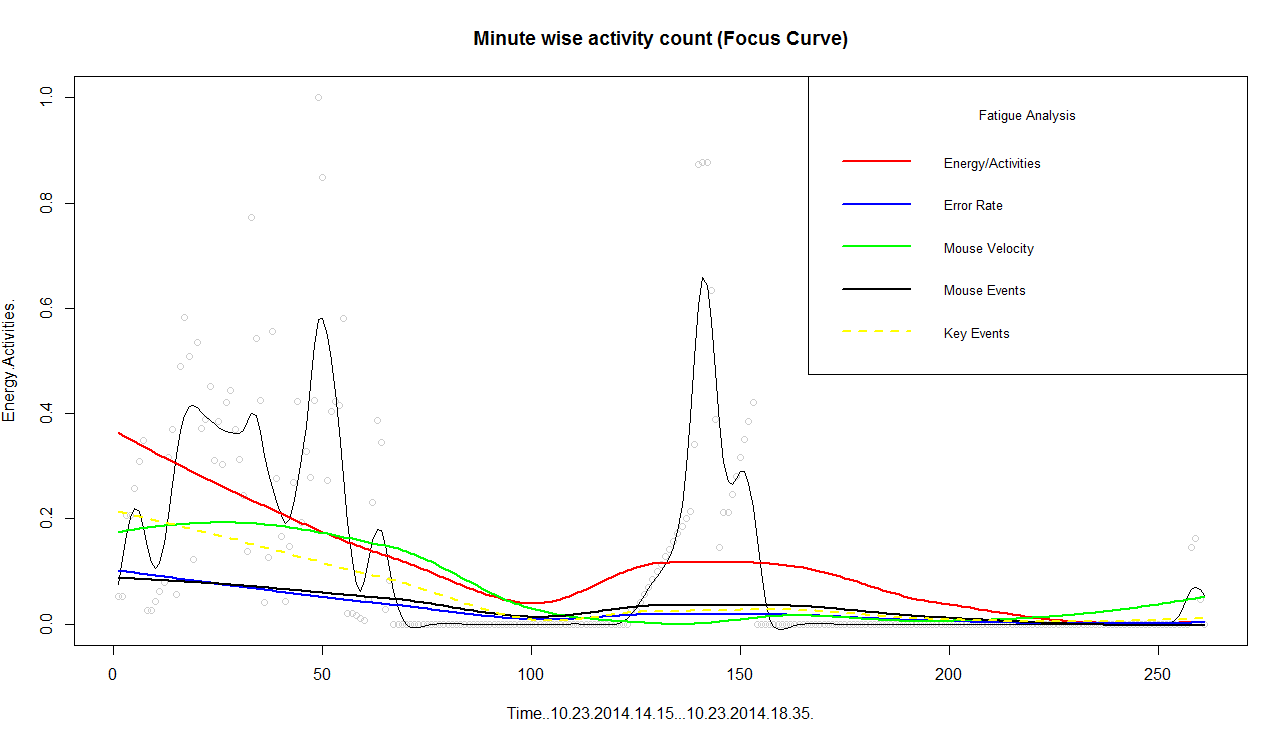
\includegraphics[width=1\textwidth,natwidth=1264,natheight=730]{focusCurve510.png}
		\caption{Focus Curve - CSC 510 Data.}
  	  \end{figure*}
  \item Data selection [TODO]
  \item Building a model and classifying mental fatigue [TODO]
  \item Observations from analysis [TODO]
  
  We intend to come up with a focus curve [Figure 7] that can show some
  working pattern of the user and build a model based on the data collected to
  classify fatigue depending on the user's activities.
\end{itemize}

\section{Study Results \& Discussion}
\begin{itemize}
  \item Discussing how the set research guidelines are used in analysis.
  \item How the user patterns \& analysis results depicts fatique, with 
  respect to the indicators.
  \item Discussion about the observations from the result and other methodologies which
can be used in order to achieve the goal.
\end{itemize}

\subsection{More Methodologies [might not include in the final draft]}
\subsubsection{In-Lab study}
\begin{itemize}
  \item The study of mental fatigue, including its causes and symptoms, is
  traditionally supported by data collected through
  instrumentation, self-reporting mechanisms (generally questionnaires) or, more
  recently, through the use of physiological sensors.
  \cite{pimenta:monitor}
  \item Specific programming tasks [TODO]
  \item We will collect data using the pre-study questionnarire, log files
  dumped by DevFatigue, and a post-study questionnaire.
  \item Electrical conductance is the method of measuring Galvanic skin response
  (GSR) monitoring sweat gland activity. We are using GSR to measure the fatigue
  activity level and validate the data collected and analysed by DevFatigue.
  \begin{itemize}
  	\item Detect
  	\item Validate
  	\item Analysis
  	\item Result
  \end{itemize}
  \item Finding patterns and setting benchmark [TODO]
\end{itemize}

\subsubsection{Industrial study}
\begin{itemize}
  \item Our research aims to help programmers avoid their fatigue state to
  control errors in programming, and eventually aid them for a better
  productivity. The application would be most suitable for the software
  industry. We have a lot of different programming tasks in an industry and
  fatigue might affect the performance/productivity of any of those
  activities. Thus, we will try conducting some studies on the real environment
  programming activities.
  \item In today's competitive world, software programmers are motivated to work
  hard, and hence keep themselves involved in numerous projects. Sometimes they
  work in teams and sometime they work individually on a project. Again, this
  all lead to sleepless nights resulting in more exhaustion and tiredness.
  \item To check the relation between mental fatigue and performance, We plan to
  review bug and code logs. My research would be taking the factors like working
  scenarios and behaviors, which affect performance, into consideration as well.
  Smith et. al. \cite{smith:coffee} studied the effects of intake of coffee on
  alertness and performance. Coetzer and Richmond \cite{richmond:team} performed
  an empirical analysis on working in teams and its relation with performance.
  \item Analysing their work patterns \& daily routines [TODO]
\end{itemize}

\section{Conclusion \& Future Work}
\begin{itemize}
\item A summary about the whole process. What all we have achieved. 
How the model and the study can be used in helping the software industry.
Talking about few contributions the study can make to the industry.
Application of the proved hypothesis.
\item After setting the baseline and recognizing fatigue states, the next step
would be to help programmers to overcome the fatigue state. It could be achieved
by various alerts, screen freezes or even suggesting Pomodoro technique. The
research is to conduct, monitor, and analyze data in a non-invasive and
non-intrusive way and present the results in a cordial manner.
\end{itemize}

\section{Acknowledgement}
Thanks to the CSC510 class at North Carolina State University for
their participation throughout the process of developing this research.

%
% The following two commands are all you need in the
% initial runs of your .tex file to
% produce the bibliography for the citations in your paper.
\bibliographystyle{abbrv}
\bibliography{doc}  % sigproc.bib is the name of the Bibliography in this case
% You must have a proper ".bib" file
%  and remember to run:
% latex bibtex latex latex
% to resolve all references
%
% ACM needs 'a single self-contained file'!
%
\balancecolumns
% That's all folks!
\end{document}
